\documentclass[a4paper]{article}
\usepackage[utf8]{inputenc}
\usepackage[russian]{babel}
\usepackage{graphicx} % для вставки изображений
\usepackage{amsmath} % для математических формул
\usepackage{hyperref} % для создания гиперссылок
\usepackage{indentfirst} % для отступа в первом абзаце секции
\usepackage[left=20mm, top=15mm, right=15mm, bottom=15mm, nohead,
footskip=10mm]{geometry} % настройки полей документа
\usepackage{minted} % для подсветки кода

\title{Модуль автомасштабирования интеллектуальных модулей для платформы MLOps}
\author{Спирин И. В., Крупнов И. И.}
\date{\today}

\begin{document}

\maketitle
\begin{abstract}
  В этом реферате рассматривается разработка модуля автоматического
  масштабирования (автоскейлинга) для интеллектуальных сервисов,
  разработанного для использования на платформе MLOps. Этот модуль
  предоставляет простой и гибкий интерфейс для управления ресурсами,
  а также поддерживает гибернацию с автоматическим восстановлением.
\end{abstract}

\tableofcontents

\section{Введение}
\subsection{Предпосылки}

Интеллектуальные модули, развертываемые на платформе, нередко нагружают
вычислительные, сетевые и дисковые ресурсы в процессе своей работы.
Причем, такое поведение наблюдается и в режиме простоя, когда модуль
не производит полезной нагрузки. Это приводит к неэффективному использованию
<<железа>>, а также может затронуть производительность сторонних программ.

Для решения этой проблемы используется автоматическое
масштабирование, которое снижает финансовые затраты как клиентов, так и
поставщиков облачных услуг.

Оркестратор Kubernetes уже предоставляет инструменты для автоскейлинга,
такие как Horizontal Pod Autoscaler (HPA), Vertical Pod Autoscaler (VPA) и
Kubernetes Event-driven Autoscaling (KEDA). Однако, они сложны в
настройке и не интегрируются с платформой напрямую. В частности, при
гибернации (полном выключении) сервиса, необходимо реализовывать
обратное восстановление вручную для каждого компонента.

\subsection{Постановка задачи}

Необходимо разработать модуль автоскейлинга для интеллектуальных сервисов,
который будет использоваться на платформе MLOps. Он должен
отслеживать использование ресурсов пользовательскими приложениями и
автоматически изменять количество реплик по значениям метрики, указанной
пользователем.

В качестве целевого объекта для масштабирования могут использоваться
Service, Deployment или ресурс MLOps-платформы MLComponent.

Также должна быть доступна возможность гибернации сервиса с
автоматическим пробуждением через стандартный API. При поступлении HTTP-запроса
на гибернированное приложение, оно должно восстанавливаться; при этом,
до готовности приложения к работе, запросы будут удерживаться, а при превышении
таймаута - должно возвращаться перенаправление (HTTP 307) на тот же URL.

Параметры таймаута и количества перенаправлений автоматически определяются по
User-Agent клиента.

\section{Архитектура}

Модуль автомасштабирования будет выполнен в виде отдельного сервиса Kubernetes,
написанного на языке Python со следующими библиотеками:

\begin{itemize}
  \item FastAPI --- для реализации асинхронного HTTP-сервера и API.
  \item kubernetes\_asyncio --- для взаимодействия с API Kubernetes в
    асинхронном режиме.
  \item APScheduler --- для создания фоновых задач на сбор метрик и
    масштабирование.
\end{itemize}

Приложение будет состоять из веб-сервера FastAPI, который будет
принимать запросы, переадресованные с гибернированных сервисов, и запросы с
менеджера оповещений. Также, в фоновом режиме будет работать планировщик
задач APScheduler, в который будут добавляться задачи на запрос
метрик из сервера метрик с последующей их обработкой.

\subsection{Структурная схема}
\begin{figure}[h]
  \centering
  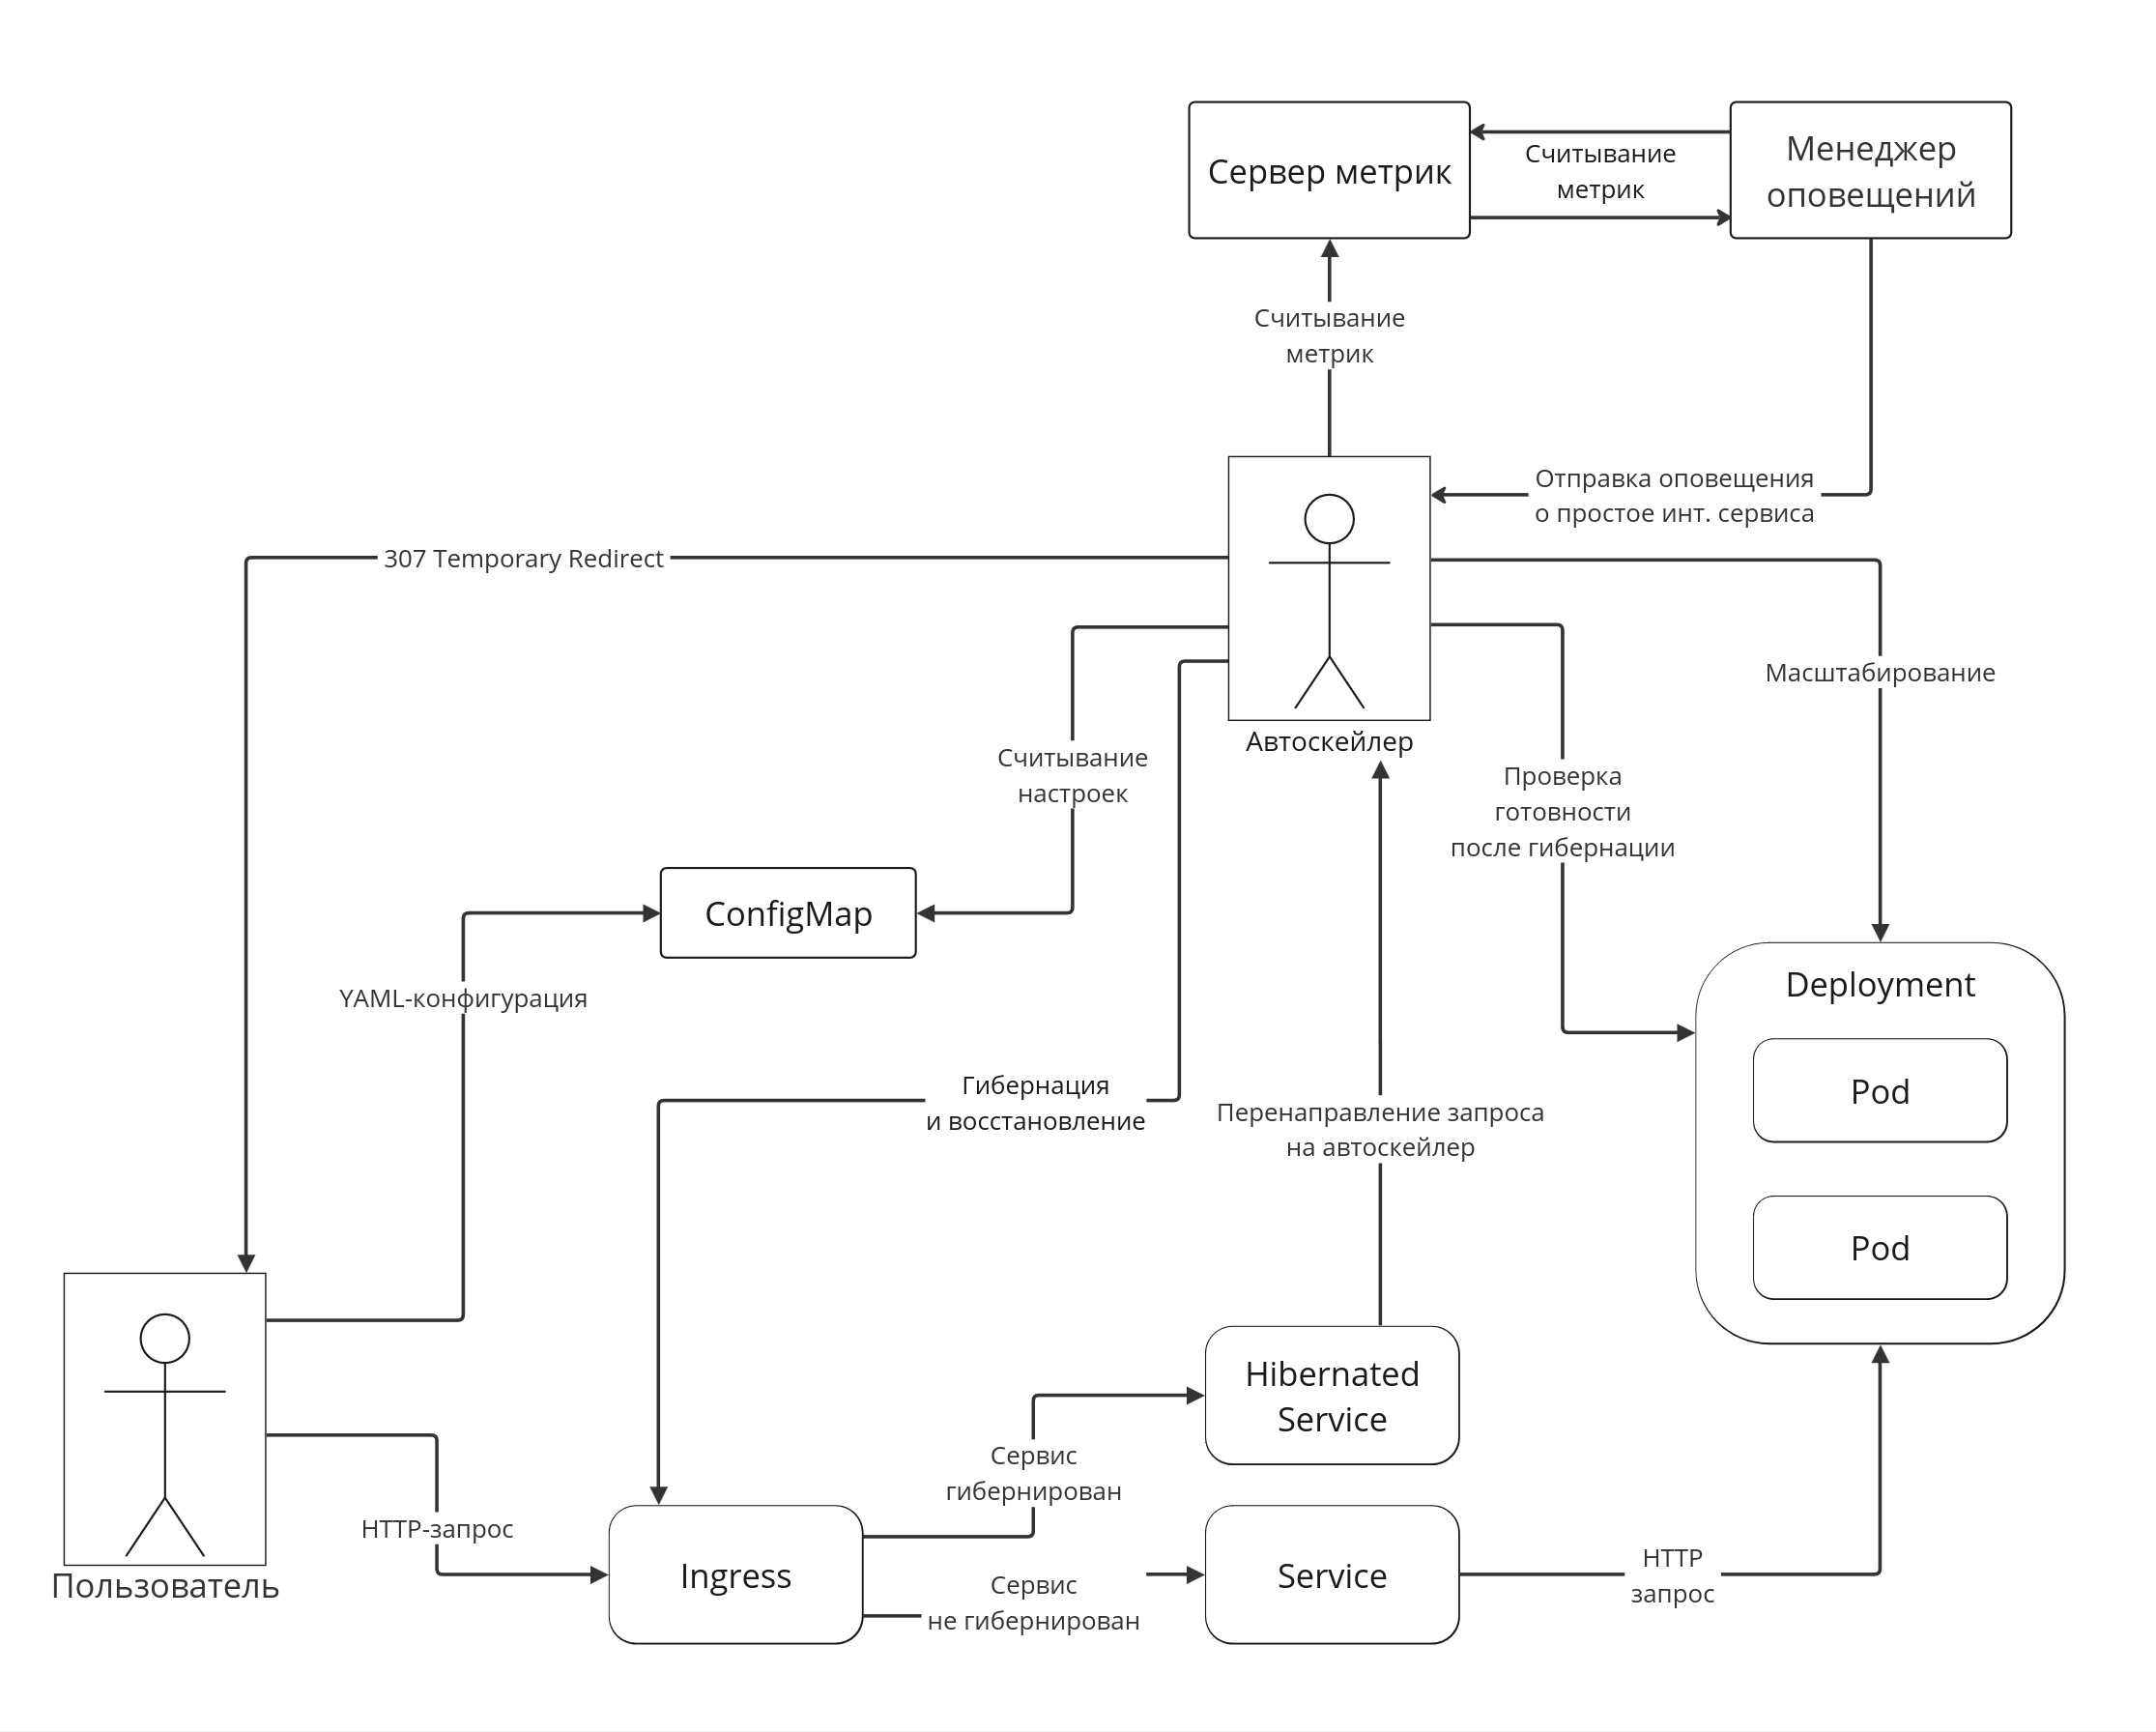
\includegraphics[width=0.8\textwidth]{img/autoscaler.jpg}
  \caption{Структурная схема модуля автоскейлинга}
  \label{fig:structure_diagram}
\end{figure}

Пользователь модуля посылает HTTP-запросы на API интеллектуального
модуля, которые приходят в общий Ingress.

При автоматической гибернации сервиса, Ingress меняется так, что
последующие запросы будут перенаправляться в автоскейлер.

Если приходит перенаправленный запрос, автоскейлер удерживает его и
запускает восстановление, после чего меняет Ingress обратно и возвращает
Redirect на тот же URL.

В фоновом режиме автоскейлер собирает метрики из сервера метрик по расписанию,
указанному в ConfigMap. Он сравнивает значения с пороговыми, и при необходимости
масштабирует Deployment интеллектуального модул.

\section{Алгоритм решения}

\subsection{Масштабирование}

В общем случае масштабирование производится с помощью изменения количества
реплик в нужном объекте Deployment с использованием API Kubernetes.
Это изменение может быть вызвано либо оповещением от сервера метрик,
либо задачей планировщика.

\subsubsection{Сервер метрик и оповещения}

Автоскейлер принимает решение о масштабировании на основании прочитанных метрик.
Для этого он формирует запросы к серверу метрик, которые должны возвращать
значения нагруженности модулей, и по расписанию собирает их.

Сервер метрик следит за состоянием кластера и развернутых на нем приложений.
Он собирает информацию об использовании ресурсов машины, о входящих и
исходящих HTTP-запросах и о многих других параметрах.

Также, такие сервера могут автоматически отправлять оповещения. Эта возможность
используется для гибернации сервиса при отсутствии запросов на API в течение
заданного времени.

\subsubsection{Масштабирование с пользовательскими параметрами}

Пользователь может указать параметры масштабирования для каждого
сервиса в объекте конфигурации ConfigMap. В таком случае,
максимальное количество реплик может превышать 1, и гибернация
сервиса будет опциональной при минимальном количестве реплик, не равном 0.

Масштабирование производится по следующему алгоритму:

\begin{enumerate}
  \item Проверка значения метрики в сервере метрик.
  \item Если пороговое значение метрики не превышено, процесс
    завершается до следующей проверки. Иначе:
  \item Поиск объектов Service, Deployment и Ingress, относящихся к сервису.
  \item Изменение количества реплик в объекте Deployment до
    значения, указанного пользователем.
\end{enumerate}

\subsubsection{Конфигурация масштабирования}

Конфигурация записывается в объект ConfigMap в формате YAML.

\begin{minted}[frame=lines,linenos=true]{yaml}
# ConfigMap для конфигурации масштабирования
apiVersion: v1
kind: ConfigMap
metadata:
  name: autoscaler-props
  namespace: unip-system-autoscaler
data:
  spec.yaml: |
    <текст spec.yaml>
\end{minted}

Файл spec.yaml содержит параметры масштабирования для каждого
сервиса, разделенные тремя дефисами.

Структура этого файла валидируется с помощью JSON Schema, которая
позволяет четко задать формат настроек (см. файл
unip\_autoscaler/autoscaling\_config.py).

В конфигурации есть несколько основных частей:

\begin{itemize}
  \item target - целевой объект масштабирования. Для каждого
    приложения, которое нужно масштабировать, указывается его имя и
    пространство имен. В поле kind указывается тип объекта -
    Deployment, Service или MLComponent.
  \item scalingRules - правила скейлинга. Здесь прописывается то, при
    каких условиях и на сколько увеличивать / уменьшать количество реплик.
    Поддерживается либо упрощенный вариант конфигурации (по средней
    загрузке CPU и RAM в среднем по всем репликам), либо использование заданной
    пользователем метрики. Масштабирование выполняется при превышении
    прописанного порогового значения.
  \item timeWindow - промежуток, за который будет собираться и
    усредняться метрика (то есть, за какой промежуток времени до текущего
    момента считать среднее значение). Используется только в случае
    задания пороговых значений CPU и RAM - предполагается, что пользовательский
    запрос будет сам включать временной промежуток и возвращать вещественное
    число.
  \item maxReplicas - максимальное количество реплик.
  \item minReplicas - минимальное количество реплик. При значении 0 доступна
    гибернация.
  \item cooldown - время в секундах, после которого не производится
    масштабирование.
\end{itemize}

\begin{minted}[frame=lines,linenos=true]{yaml}
# Пример spec.yaml
target:
  kind: deployment
  name: student-chatbot-mlcmp-deployment
  namespace: pu-test-pa-student-chatbot
scalingRules:
  scaleUp:
    step: 2  # сколько реплик добавлять
    # нужно указать хотя бы один из порогов cpuThreshold, memoryThreshold
    # ЛИБО метрику из Prometheus
    # Prometheus-запрос для этого соберется автоматически
    cpuThreshold: 50  # пороговое использование CPU, %
    memoryThreshold: 500  # пороговое использование памяти, МБ
  scaleDown:
    step: 1 # сколько реплик убирать
    cpuThreshold: 10
    memoryThreshold: 200
timeWindow: 300  # время в секундах, в течение которого собираются метрики
maxReplicas: 10  # максимальное количество реплик
minReplicas: 0  # минимальное; параметр minReplicas=0 включает гибернацию
cooldown: 300  # время в секундах, после которого возможно повторное масштабирование
---
target:
  kind: deployment
  name: pythonserver
  namespace: unip-system-autoscaler
scalingRules:
  prometheusMetric:
    query: |
      sum by (pod) (rate(
        container_cpu_usage_seconds_total{pod=~"pythonserver-.*"}[1m]
      )) * 100
    thresholdUp: 50  # пороговое значение, при превышении которого сервис масштабируется вверх
    thresholdDown: 25  # то же самое, но вниз
    stepUp: 1  # на сколько реплик увеличивать
    stepDown: 1  # на сколько реплик уменьшать
maxReplicas: 3
minReplicas: 1
cooldown: 120
\end{minted}

\subsubsection{Гибернация и восстановление}

В режиме работы по умолчанию гибернация производится после оповещения
от AlertManager (менеджера оповещений) об отсутствии запросов на API
интеллектуального сервиса в течение заданного времени.

Количество реплик уменьшается до 0, и следующий запрос переадресуется
в автоскейлер.

Гибернация производится по следующему алгоритму:

\begin{enumerate}
  \item Получение запроса на гибернацию сервиса.
  \item Поиск объектов Service, Deployment и Ingress, относящихся к сервису.
  \item Поиск объекта Service с суффиксом <<-hibernated>>; при
    отсутствии, его создание.
  \item Изменение объекта Ingress для перенаправления HTTP-запросов на
    автоскейлер.
  \item Изменение объекта Deployment для уменьшения количества реплик до 0.
\end{enumerate}

Восстановление производится по следующему алгоритму:

\begin{enumerate}
  \item Получение запроса на восстановление в сервис с суффиксом
    <<-hibernated>>.
  \item Поиск объектов Service, Deployment и Ingress, относящихся к сервису.
  \item Изменение количества реплик в объекте Deployment до
    изначального значения.
  \item Запуск цикла для проверки готовности сервиса, во время
    которого перехваченный HTTP-запрос будет удерживаться, и при
    истечении таймаута будет возвращаться переадресация со статусом
    307 Temporary Redirect на тот же URL.
  \item Изменение объекта Ingress до изначального состояния.
  \item Переадресация запроса на восстановленный сервис.
\end{enumerate}

\begin{figure}[h]
  \centering
  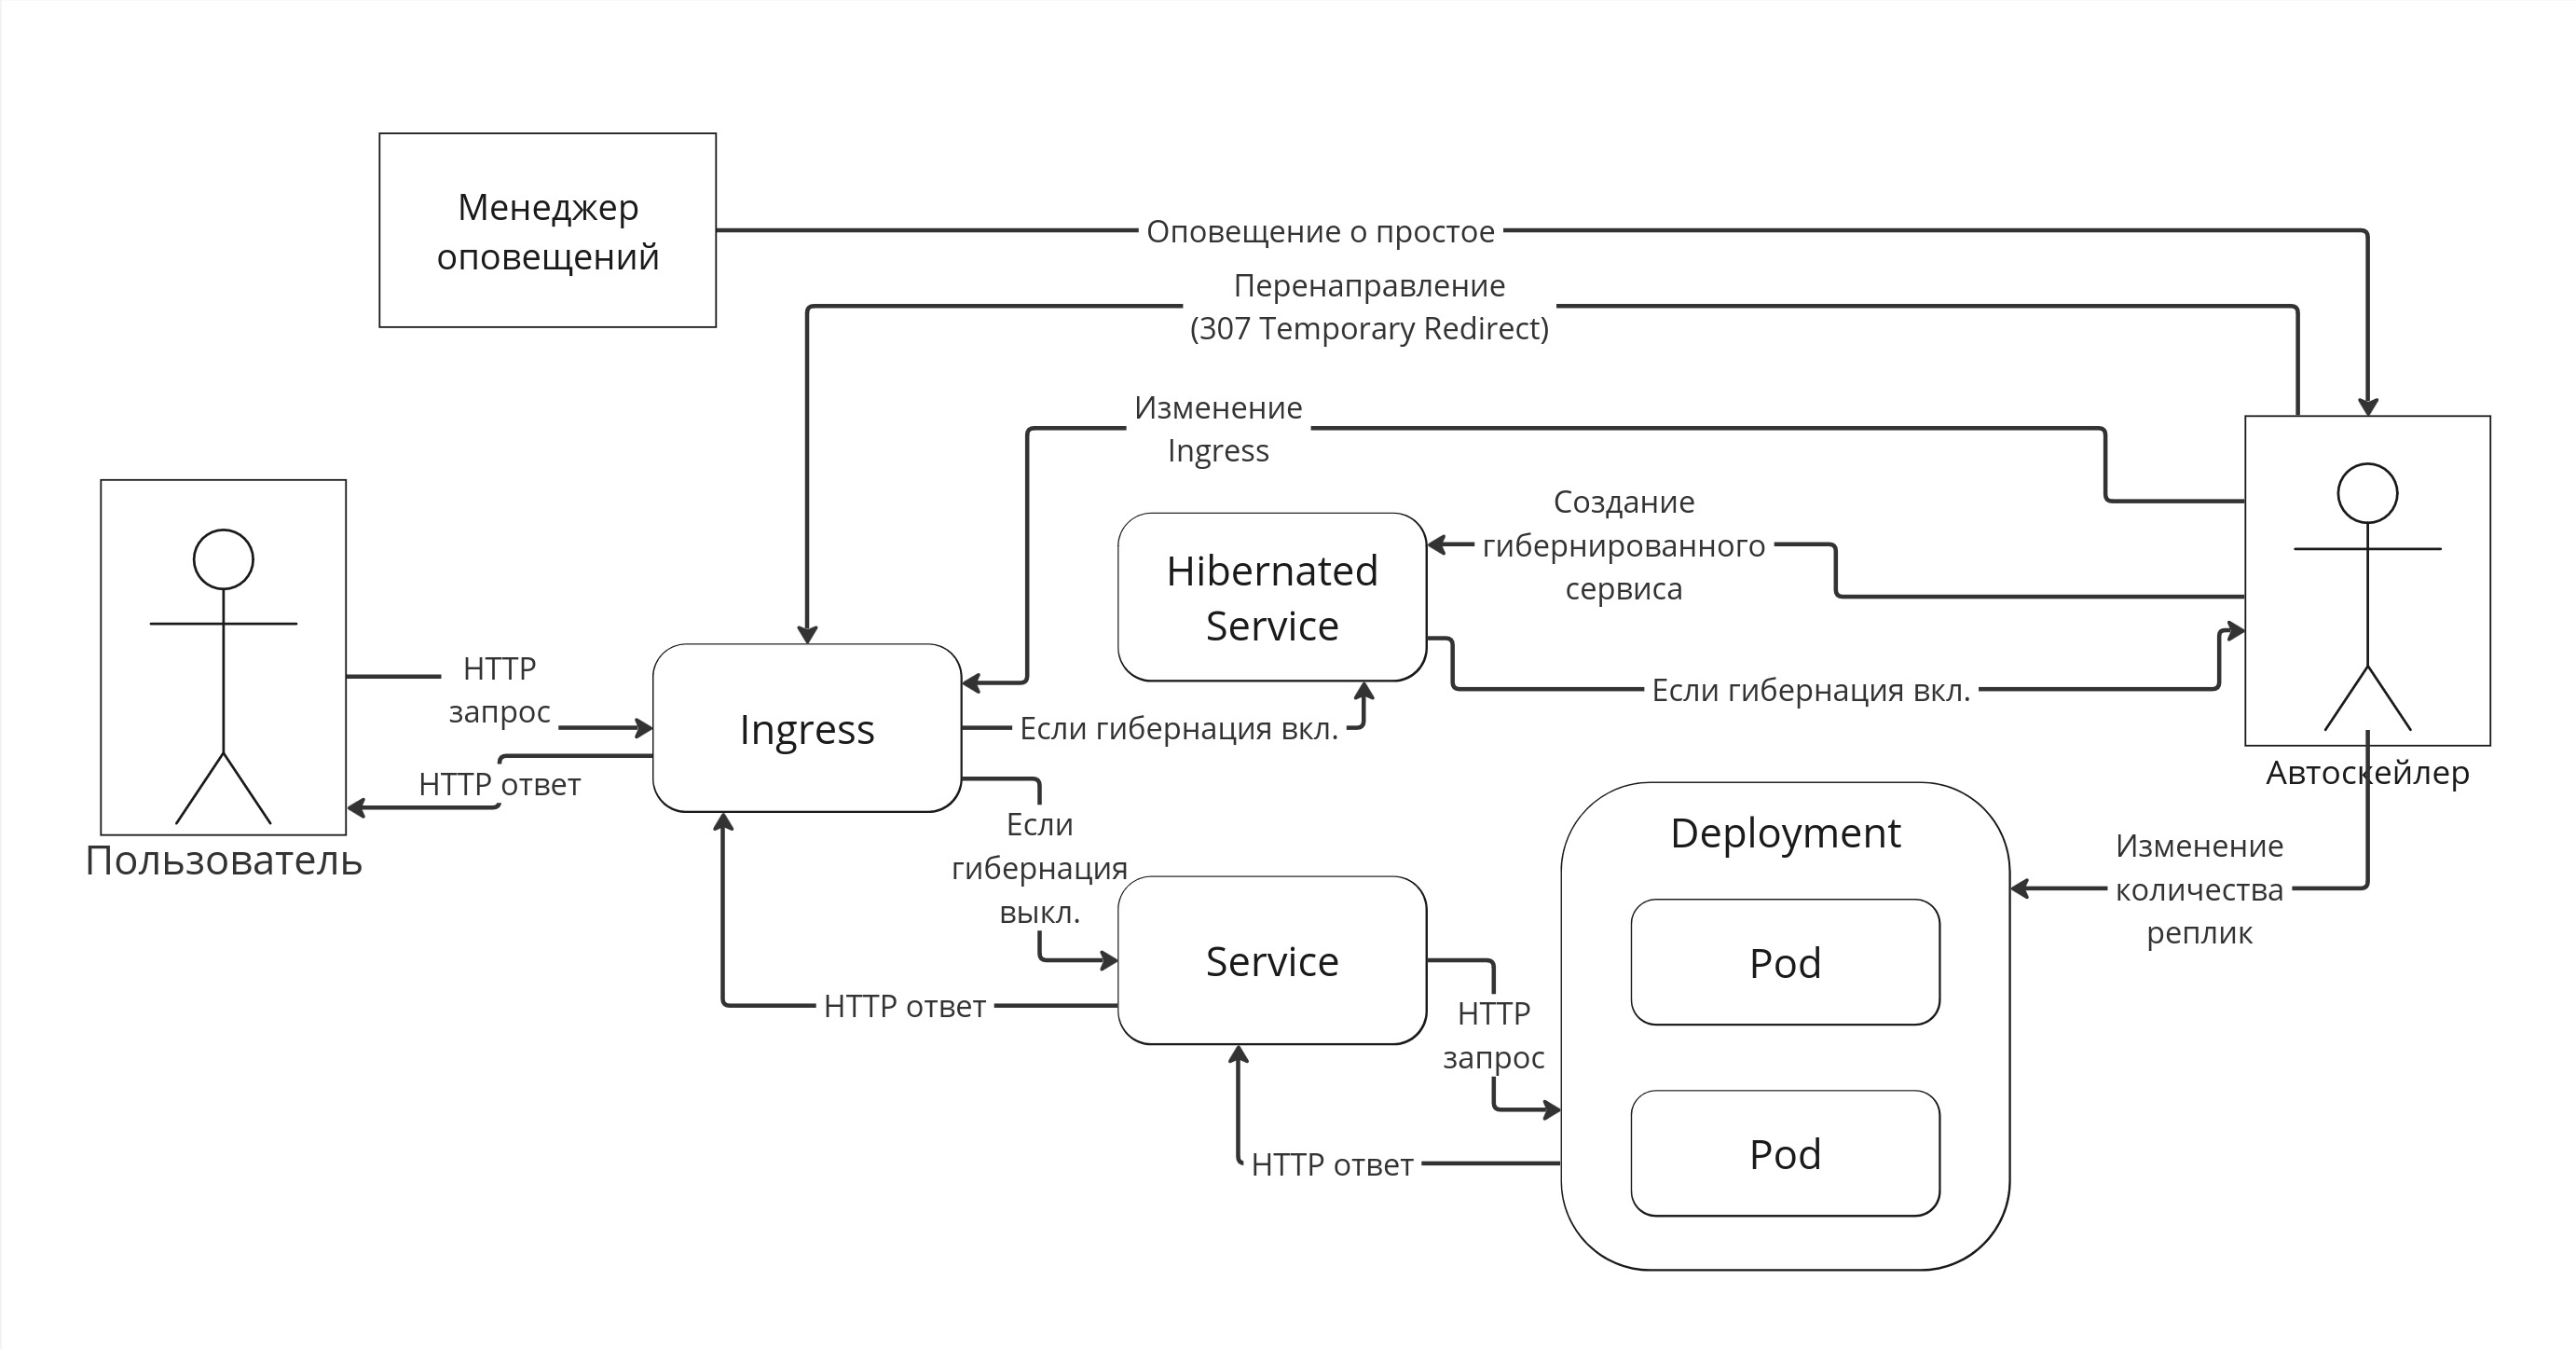
\includegraphics[width=0.8\textwidth]{img/hibernate-restore.jpg}
  \caption{Структурная схема гибернации и восстановления}
  \label{fig:hibernate_diagram}
\end{figure}


\section{Тестирование}
\subsection{Протокол тестирования}
Для проверки работы модуля были проведены тесты, которые включали в себя:

\begin{enumerate}
  \item Тестирование гибернации и восстановления MLComponent c
    проверкой запросов на APIComponent
  \item Тестирование масштабирования Deployment стресс-теста с
    заданными порогами CPU и памяти (и отдельно с запросом в
    сервер метрик).
\end{enumerate}

\subsubsection{Тестирование гибернации и восстановления}

\begin{enumerate}
  \item Запустить MLComponent с рабочей функцией inference (см.
    репозиторий mlops\_platform/demo-project).
  \item Подождать определенное время до гибернации (по умолчанию 5 минут).
  \item Проверить, что в Ingress сервиса записались дополнительные правила
    для перенаправления на автоскейлер.
  \item Проверить, что создан сервис-заглушка с суффиксом <<-hibernated>>.
  \item Проверить, что количество реплик Deployment равно 0.
  \item Послать запрос на инференс через Postman (или другой HTTP-клиент).
  \item Убедиться, что в логах автоскейлера появилось сообщение о
    восстановлении.
  \item Подождать, пока сервис не станет доступен и проверить
    количество реплик.
  \item Проверить, что результат HTTP-запроса верный.
\end{enumerate}

\subsubsection{Тестирование масштабирования Deployment}

\begin{enumerate}
  \item Запустить тестовый Deployment с приложением stress-ng (см.
    файл k8s/stress-ng.yaml).
  \item Дождаться обновления значений CPU/RAM в сервере метрик.
  \item Проверить, что количество реплик увеличилось до заданного значения.
  \item Дождаться окончания работы стресс-теста во всех репликах.
  \item Проверить, что количество реплик уменьшилось до
    минимального значения.
  \item Повторить шаги выше с запросом в сервер метрик и
    приложением на Python
    (см. файл k8s/python.yaml).
\end{enumerate}

\subsection{Параметры тестирования}

В процессе тестирования для сборки образов использовались следующие версии:

\begin{itemize}
  \item Python версии 3.12
  \item Kubernetes версии 1.29
  \item Операционная система: Ubuntu 20.04
\end{itemize}

\section{Ссылки на репозитории}

\begin{itemize}
  \item Репозиторий с исходным кодом модуля автоскейлинга:
    \href{https://platform.stratpro.hse.ru/forgejo/ispirin/unip-autoscaler}{ispirin/unip-autoscaler}
  \item Репозиторий с тестовым модулем:
    \href{https://platform.stratpro.hse.ru/forgejo/mlops_platform/demo-project}{mlops\_platform/demo-project}
\end{itemize}

\end{document}
